Deriving the equations of motion to predict the movement of a satellite around a Lagrange point will be much more difficult than locating the Lagrange points.
We will need to come up with a coordinate system that we can use to define our equations of motion around, as well as specific parameters for the physical system to allow the mathematics to be easier. \par
\begin{wrapfigure}{l}{0.6\textwidth}
	\centering
	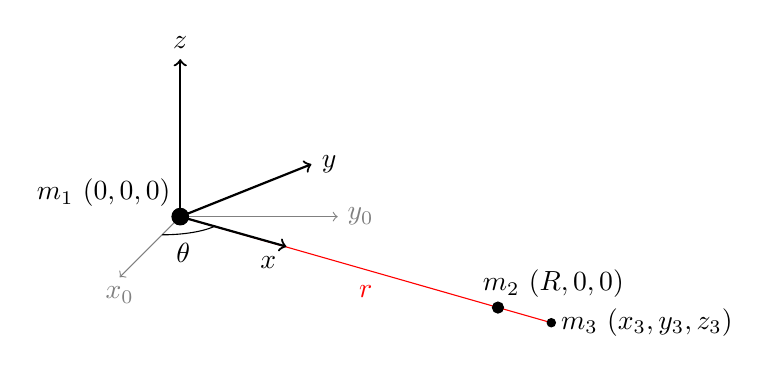
\begin{tikzpicture}
		\coordinate (o) at (0,0,0);
		\draw[thin,gray,->] (0,0,0) -- (0,0,2) node[below] {$\uvec{x}_0$};
		\draw[thin,gray,->] (0,0,0) -- (2,0,0) node[right] {$\uvec{y}_0$};
		
		\draw[red] (o) -- (6.06,0,3.5) node[midway,yshift=-8pt]{$\bvec{r}$};
		
		\draw[thick,->] (0,0,0) -- (0,2,0) node[above] {$\uvec{z}$};
		\draw[thick,->] (0,0,0) -- (1.73,0,0.99) node[below left] {$\uvec{x}$};
		\draw[thick,->] (0,0,0) -- (1,0,-1.73) node[right] {$\uvec{y}$};
		
		\draw (0,0,0.6) arc [start angle=-90,end angle=-32,x radius=0.8,y radius=0.24];
		\node at (.5,0,1.2) {$\theta$};
		
		\filldraw (0,0,0) circle (3pt) node[above left] {$m_1$ $(0,0,0)$};
		\filldraw (5.19,0,3) circle (2pt) node[above,xshift=20pt] {$m_2$ $(R,0,0)$};
		\filldraw (6.06,0,3.5) circle (1.5pt) node[right] {$m_3$ $(x_3,y_3,z_3)$};
	\end{tikzpicture}
	\vspace*{0.25cm}
	\caption{three-dimensional diagram of the Sun-Earth system with unit vectors relative to the Earth's orbit. Not drawn to scale.}
	\label{fig:3d-coords}
\end{wrapfigure}
Firstly, we must assert that $m_1 \gg m_2$, meaning that the movement of the Sun due to the gravity of Earth is negligible.
This allows the Sun to be placed at the center of the coordinate system, avoiding the need to make considerations for the center of mass of the system.
It is also asserted that $m_2 \gg m_3$, so that, similarly to the previous assertion, the satellite has a negligible effect on Earth.
Secondly, continuing with the conditions from the previous calculations, it is assumed that the Earth is in a circular orbit, making the system a little easier to comprehend.
Thirdly, and unlike the previous calculations, we will derive the equations of motion from a inertial reference frame, meaning that we will not be viewing this system from a moving point of reference.
This will allow us to completely determine motion without the need to consider fictitious forces.

As shown in Figure \ref{fig:3d-coords}, we will have unit vectors $\uvec{x}$, $\uvec{y}$, and $\uvec{z}$ drawn relative to the orbit of the Earth.
The satellite around L2, $m_3$, will have the coordinates $(x_3,y_3,z_3)$ represented by the vector $\bvec{r}$.
Taking from my understanding of vectors, the position of a satellite can be expressed as:
\begin{equation*}
	\bvec{r} = x_3\uvec{x} + y_3\uvec{y} + z_3\uvec{z}
\end{equation*}
Because the unit vectors are not actually static in the system ($\uvec{x}$ and $\uvec{y}$ rotate about the origin), their movement must be taken into account.
\begin{gather*}
	\uvec{x} = (\cos\theta)\uvec{x}_0 + (\sin\theta)\uvec{y}_0 \\
	\uvec{y} = -(\sin\theta)\uvec{x}_0 + (\cos\theta)\uvec{y}_0 \\
	\uvec{z} = \uvec{z}_0
\end{gather*}
At this point, it is crucial to notice that these equations are not yet useful to us to describe movement.
In order to describe motion, we need to be able to define the velocity and acceleration of the satellite in three-dimensional space.
This means being able to take the derivative of a vector.
Let us assert the following axiom, for some vector \textbf{v} with the basis vectors $\uvec{i}$ and $\uvec{j}$ components $a$ and $b$:
\begin{equation}
	\frac{d\bvec{v}}{dt} = \frac{da}{dt}\uvec{i} + \frac{db}{dt}\uvec{j}
\end{equation}
In other words, the derivative of a vector is the derivative of its components, and would be consistent with the sum rule for derivatives. 
The notation here can become quite bloated and difficult to read if we continue to use Leibniz's notation.
So instead, from here on, we will use Newton's notation where possible.

We can take the second derivative of our position vector $\bvec{r}$:
\begin{equation*}
	\bvec{a} = \frac{d^2\bvec{r}}{dt^2} = \frac{d^2x_3\uvec{x}}{dt^2} + \frac{d^2y_3\uvec{y}}{dt^2} + \frac{d^2z_3\uvec{z}}{dt^2}
\end{equation*}
Our acceleration vector is then expanded to:
\begin{equation*}
	\bvec{a} = \ddot{x}_3\uvec{x} + 2\dot{x}_3\dot{\uvec{x}} + x_3\ddot{\uvec{x}} + \ddot{y}_3\uvec{y} + 2\dot{y}_3\dot{\uvec{y}} + x_3\ddot{\uvec{y}} + \ddot{z}_3\uvec{z} + 2\dot{z}_3\dot{\uvec{z}} + z_3\ddot{\uvec{z}}
\end{equation*}